\documentclass[a4paper,11pt]{article}
\usepackage[utf8]{inputenc}
\usepackage{amsmath}
\usepackage{amsfonts}
\usepackage{amssymb}
\usepackage{graphicx}
\usepackage{braket}

\numberwithin{equation}{section}
\renewcommand\thesubsection{\alph{subsection}}
\newcommand{\bvp}[1]{\mathbf{#1}'}
\newcommand{\bv}[1]{\mathbf{#1}}
\newcommand{\ez}{\epsilon_0}
\newcommand{\eo}{\epsilon_1}
\newcommand{\lrp}[1]{\left({#1}\right)}
\newcommand{\lrb}[1]{\left\{{#1}\right\}}


%opening
\title{Computational Biophysics HW5}
\author{Vince Baker}

\begin{document}

\maketitle

\section{Question 1}
We first derive the dimensionless potentials:
\begin{align}
 V_{00} &= 4\ez\lrp{\lrp{\frac{\sigma_0}{r}}^{12}-\lrp{\frac{\sigma_0}{r}}^{6}}\\
 \sqrt{\ez\eo}V'_{00} &= 4\ez\lrp{\lrp{\frac{\sigma_0}{r\sigma_0}}^{12}-\lrp{\frac{\sigma_0}{r\sigma_0}}^{6}}\\
 V'_{00} &= 4\sqrt{\frac{\ez}{\eo}}\lrp{\lrp{\frac{1}{r}}^{12}-\lrp{\frac{1}{r}}^{6}}\\
  V_{01} &= 4\sqrt{\ez\eo} \lrp{\lrp{\frac{\sigma_0+\sigma_1}{2}\frac{1}{r}}^{12}-\lrp{\frac{\sigma_0+\sigma_1}{2}\frac{1}{r}}^{6}}\\
 \sqrt{\ez\eo}V'_{01} &= 4\sqrt{\ez\eo} \lrp{\lrp{\frac{\sigma_0+\sigma_1}{2\sigma_0}\frac{1}{r}}^{12}-\lrp{\frac{\sigma_0+\sigma_1}{2\sigma_0}\frac{1}{r}}^{6}}\\
 V'_{01} &= 4\lrp{\lrp{\frac{\sigma_0+\sigma_1}{2\sigma_0}\frac{1}{r}}^{12}-\lrp{\frac{\sigma_0+\sigma_1}{2\sigma_0}\frac{1}{r}}^{6}}\\
 V_{11} &= 4\eo\lrp{\lrp{\frac{\sigma_1}{r}}^{12}-\lrp{\frac{\sigma_1}{r}}^{6}}\\
 \sqrt{\ez\eo}V'_{11} &= 4\eo\lrp{\lrp{\frac{\sigma_1}{r\sigma_0}}^{12}-\lrp{\frac{\sigma_1}{r\sigma_0}}^{6}}\\
 V'_{11} &= 4\sqrt{\frac{\eo}{\ez}}\lrp{\lrp{\frac{\sigma_1}{\sigma_0 r}}^{12}-\lrp{\frac{\sigma_1}{\sigma_0 r}}^{6}}
\end{align}
We now derive the dimensionless acceleration as the derivative of the negative potential:
\begin{align}
 |\ddot{r}_{00}| &= 48\sqrt{\frac{\ez}{\eo}}\lrp{ \lrp{\frac{1}{r}}^{13}-\frac{1}{2}\lrp{\frac{1}{r}}^{7} }\\
 |\ddot{r}_{01}| &= 48\lrp{ \lrp{\frac{\sigma_0+\sigma_1}{2\sigma_0}}^{12}\lrp{\frac{1}{r}}^{13}-\lrp{\frac{\sigma_0+\sigma_1}{2\sigma_0}}^{6}\lrp{\frac{1}{r}}^{7} }\\
 |\ddot{r}_{11}| &= 48\sqrt{\frac{\eo}{\ez}}\lrp{ \lrp{\frac{\sigma_1}{\sigma_0}}^{12}\lrp{\frac{1}{r}}^{13}-\lrp{\frac{\sigma_1}{\sigma_0}}^{6}\frac{1}{2}\lrp{\frac{1}{r}}^{7} }
\end{align}
To find the total energy we need a dimensionaless expression for the kinetic energy of each particle. 
The transformation to dimensionless coordinates results in $v = \frac{dr}{dt} = \sqrt{\frac{\sqrt{\ez\eo}}{m}}$.
The dimensionless kinetic energy of each particle can then be written:
\begin{align}
 K &= \frac{\sqrt{\ez\eo}}{6}\lrp{v_x^2+v_y^2+v_z^2}
\end{align}
Using the equipartition theorem, $\frac{3}{2}k_B T = K$, so the temperature in units of $(\sqrt{\ez\eo})/k_B$ is $\frac{1}{9}\lrp{v_x^2+v_y^2+v_z^2} $.
\\ \\
\section{Computer Experiment}
For each of 7 densities (0.2, 0.3, 0.4, 0.5, 0.6, 0.7, 0.845) the collision times were captured.
The collision times were grouped into a 100-point histogram, and the log of the histogram was plotted up to the first zero value.
A sample graph is shown in figure 1.\\
\begin{figure}[h]
 \caption{Semilog graph for density 0.3}
 \centering
   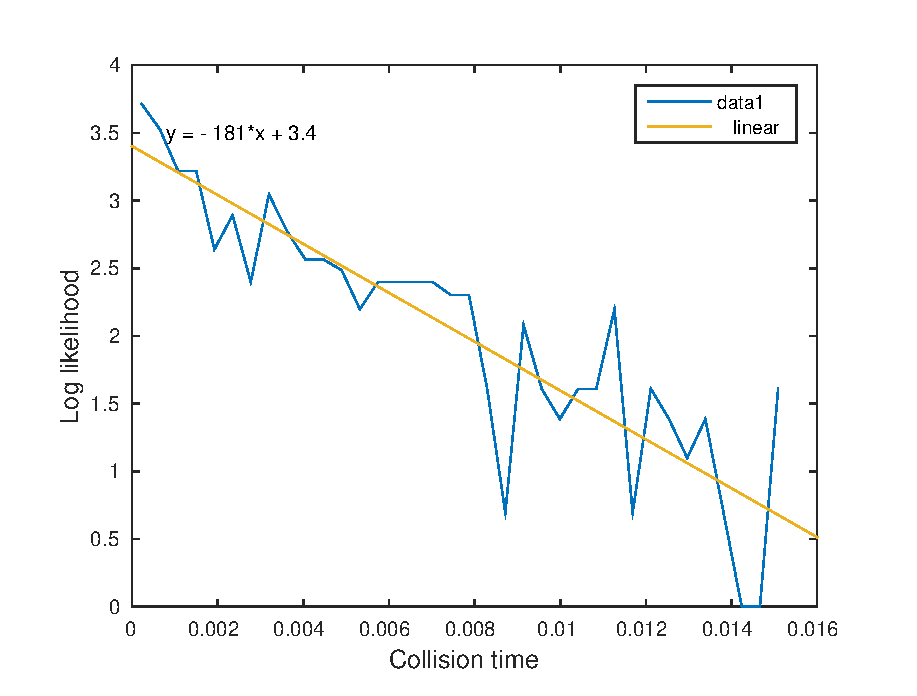
\includegraphics[width=\textwidth]{hist_d03}
\end{figure}
\\
The linear fit to this semilog graph provides the $\lambda$ parameter for the exponential distribution (PDF $\lambda e^{-\lambda})$.
The mean value of the distribution is $-1/\lambda$, which is the characteristic time plotted below in figure 2. 
For densities less than about 0.3 the mean collision time in the DMD code will be shorter than the MD time step, so we can reasonably expect the DMD code to be faster.
\begin{figure}[h]
 \caption{Characteristic collision times}
 \centering
   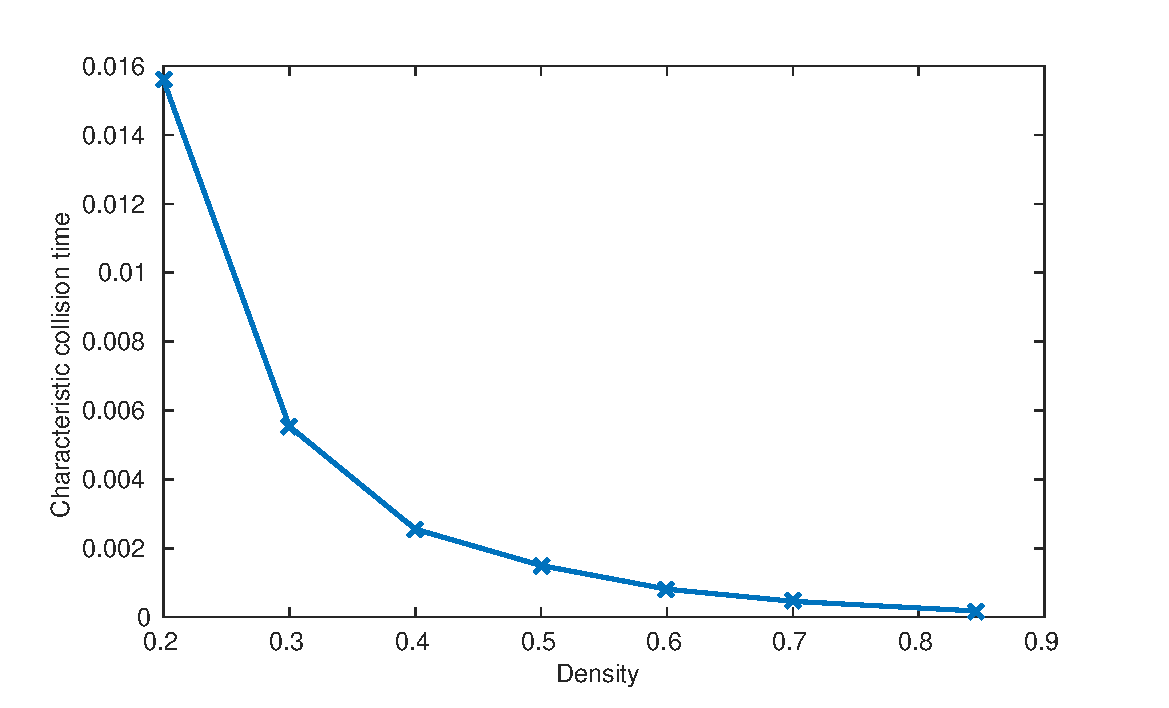
\includegraphics[width=\textwidth]{collisionTimes}
\end{figure}



\end{document}
